\documentclass[11pt,a4paper]{ctexart}
\usepackage[margin=2.15cm]{geometry}
\usepackage{amsmath,amssymb,bm,booktabs,array,graphicx,xcolor,hyperref,siunitx,longtable}
\usepackage{caption,enumitem}
\hypersetup{colorlinks=true,linkcolor=blue!55!black,urlcolor=blue!55!black}
\graphicspath{{../results/}}
\setlength{\parindent}{2em}
\setlength{\parskip}{0.25em}
\setlist{nosep,leftmargin=2.2em}
\title{EXP-017：高频变压器端口观测下的\\Fisher/OED 与可辨识参数子空间}
\author{高频变压器智能建模实验链}
\date{2026年9月9日}

\begin{document}
\maketitle

\begin{abstract}
EXP-016 已证明图网络和可微矩阵物理链路能够运行，但八个结构化尺度在几乎零响应残差下仍出现约 $7.16\%$ 的平均尺度误差，Jacobian 条件数约为 $1369$。本实验不继续增加神经网络复杂度，而是使用 EXP-015 的精确矩阵/Kron 求解器，系统计算八个对数参数对 $Y_{11},Y_{22},Y_{12}$ 在 12 个频点上的 Jacobian 和 Fisher 信息。随后比较全八参数、Fisher 选择的四个原参数、四维主可辨识子空间三种局部反演，并比较六个均匀频点与六个贪心 log-det OED 频点。100 次含噪 Monte Carlo 表明：单一端口在数值上严重病态；联合三端口和 OED 显著改善最小奇异值；在当前噪声和局部扰动范围内，OED 加四维低秩参数子空间将平均参数误差由全八参数的 $12.59\%$ 降至 $3.20\%$。结论只适用于合成 8+8 分段参考模型，不构成 DAB、FEM 或实物结论。
\end{abstract}

\section{实验位置与问题来源}
本实验使用三层已有成果：EXP-015 提供图到 $\bm R,\bm L,\bm C,\bm G$ 的转换及精确 Kron 消元；EXP-016 提供八个正值结构尺度及其可微参数化；EXP-017 研究端口观测究竟能稳定辨识哪些参数或参数组合。八个参数为
\begin{equation}
\bm z=[z_{R_p},z_{R_s},z_{L_\sigma},z_{L_m},z_{C_{lp}},z_{C_{ls}},z_{C_g},z_{C_{ps}}]^\mathsf{T},
\qquad s_i=\exp(z_i)>0.
\end{equation}
指数映射保证尺度为正；$\bm L=s_{L_\sigma}\bm L_\sigma+s_{L_m}\bm L_m$ 保持正定结构，电容子矩阵的非负组合保持半正定结构。

本实验的核心问题不是``能否把频响拟合得很小''，而是：当测量含噪时，是否存在不同的 $\bm z$ 产生几乎相同的端口频响。若存在，则端口响应误差小不能等价为每个内部参数正确。

\section{精确物理教师与观测向量}
对每个角频率 $\omega$，分段网络的节点导纳为
\begin{equation}
\bm Y_n(\omega)=\bm A(\bm R+j\omega\bm L)^{-1}\bm A^\mathsf{T}+\bm G+j\omega\bm C.
\end{equation}
将外部端口节点记为 $p$、内部节点记为 $i$，Kron 消元得到
\begin{equation}
\bm Y_{\mathrm{port}}=\bm Y_{pp}-\bm Y_{pi}\bm Y_{ii}^{-1}\bm Y_{ip}.
\end{equation}
程序实际使用线性方程求解而不显式求逆。对每个频点提取 $Y_{11},Y_{22},Y_{12}$，观测采用幅相形式
\begin{equation}
\bm h_k=\bigl[\log_{10}|Y_{11}|,\log_{10}|Y_{22}|,\log_{10}|Y_{12}|,
\angle Y_{11},\angle Y_{22},\angle Y_{12}\bigr]^\mathsf{T}.
\end{equation}
12 个对数频点覆盖 \SI{10}{kHz}--\SI{10}{MHz}，完整观测维数为 $72$。

\section{Jacobian、Fisher 信息与病态性}
在标称点 $\bm z_0=\bm 0$ 处用 PyTorch 自动微分计算
\begin{equation}
\bm J_k=\left.\frac{\partial\bm h_k}{\partial\bm z}\right|_{\bm z_0},\qquad
\bm F=\sum_k\bm J_k^\mathsf{T}\bm W_k\bm J_k.
\end{equation}
本次合成试验设同方差白噪声，故 $\bm W_k$ 与单位阵成比例。由于 $z_i$ 已是无量纲相对尺度，主 Fisher 分析保留 Jacobian 原始列范数；若将每列强制单位化，会抹去弱参数本身信息不足这一事实。代码仍保存列归一化 Jacobian，供复核，但不用于主结论。

若 $\bm J=\bm U\bm\Sigma\bm V^\mathsf{T}$，则 $\sigma_{\min}$ 衡量最弱可见方向，$\kappa=\sigma_{\max}/\sigma_{\min}$ 衡量噪声放大。形式满秩并不意味着可稳定反演；当 $\sigma_{\min}$ 极小时，系统虽有秩 8，实际仍近似不可辨识。

\begin{table}[htbp]
\centering
\caption{不同端口组合的局部可辨识性}
\begin{tabular}{lrrr}
\toprule
观测 & 秩 & $\sigma_{\min}$ & 条件数 $\kappa$\\
\midrule
$Y_{11}$ & 8 & $1.62\times10^{-10}$ & $1.97\times10^{10}$\\
$Y_{22}$ & 8 & $2.40\times10^{-9}$ & $6.62\times10^{8}$\\
$Y_{12}$ & 8 & $5.78\times10^{-11}$ & $2.74\times10^{10}$\\
$Y_{11}+Y_{22}$ & 8 & $9.05\times10^{-5}$ & $3.87\times10^{4}$\\
三端口、12频点 & 8 & $1.71\times10^{-3}$ & $2.22\times10^{3}$\\
\bottomrule
\end{tabular}
\end{table}

表中最重要的结果是：单端口即使被数值秩判为 8，其条件数仍达到 $10^9$--$10^{10}$，因此不应表述为``八参数可辨识''。互导纳 $Y_{12}$ 对跨绕组耦合重要，但它不能独自区分全部八参数；三端口互补才将条件数降低约六至七个数量级。

\section{频点 OED}
从 12 个候选频点中选 6 个。均匀方案选取索引 $[0,2,4,7,9,11]$。OED 使用带微小岭项的贪心 log-det 准则：
\begin{equation}
f^*=\arg\max_{f\notin\mathcal F}
\log\det\left(\epsilon\bm I+
\sum_{q\in\mathcal F\cup\{f\}}\bm J_q^\mathsf{T}\bm J_q\right),
\qquad \epsilon=10^{-6}.
\end{equation}
最终选择 \SIlist{10;18.738;35.112;65.793}{kHz}、\SI{5.337}{MHz} 和 \SI{10}{MHz}。它保留低频电阻/磁支路信息与高频电容信息，而不是平均铺满频带。

\begin{figure}[htbp]
\centering
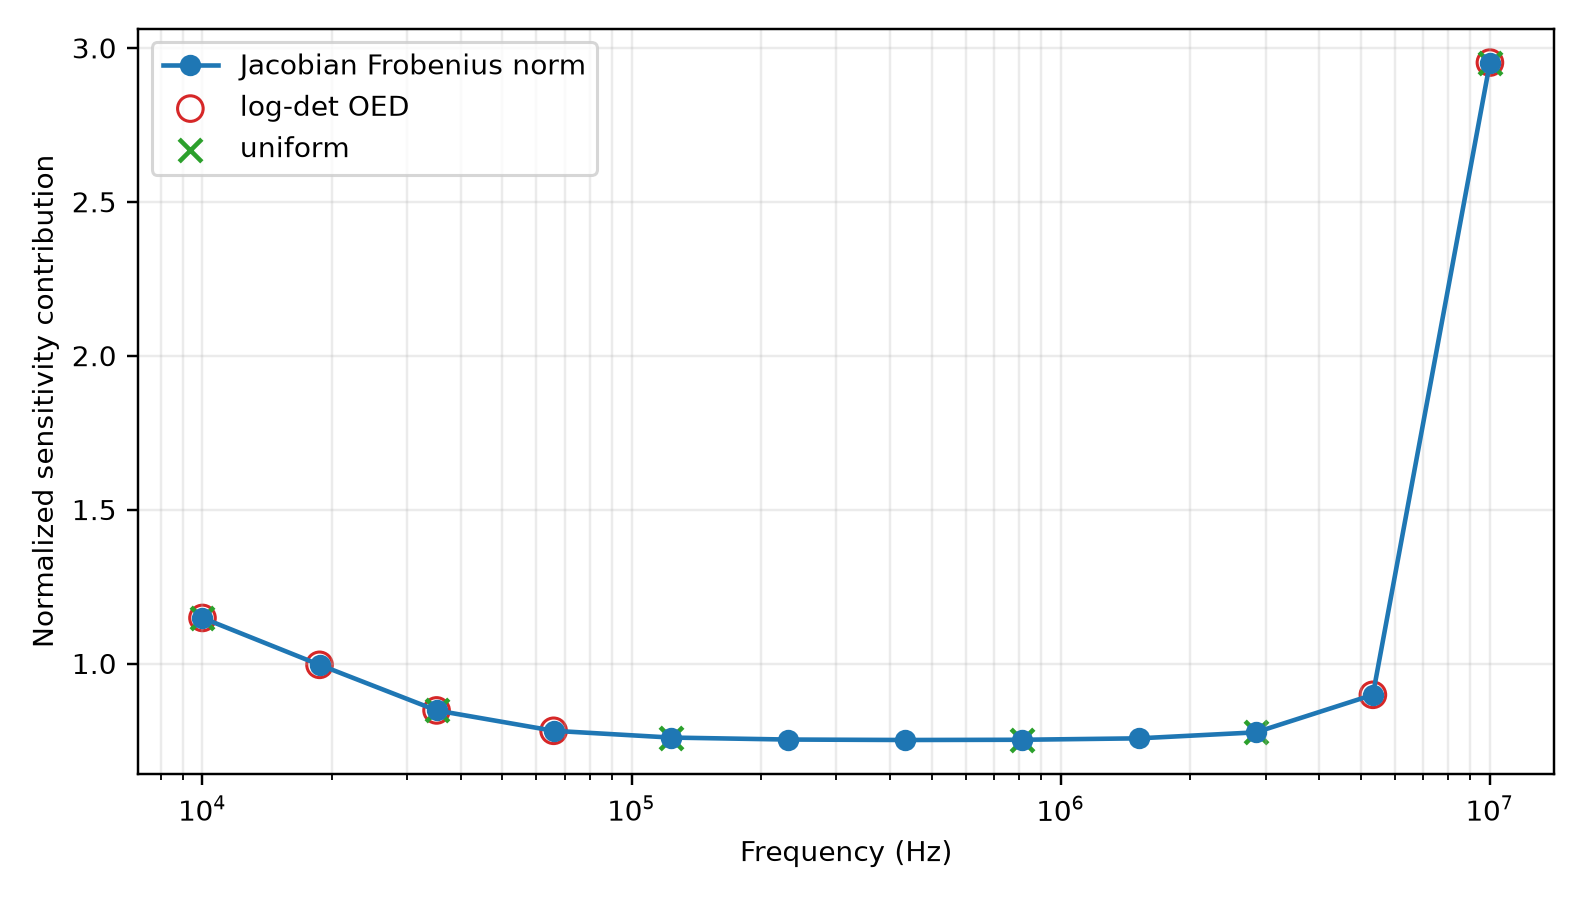
\includegraphics[width=.82\linewidth]{frequency_selection.png}
\caption{逐频点灵敏度贡献、均匀频点与 log-det OED 频点。}
\end{figure}

六个均匀频点的 $\sigma_{\min}=4.82\times10^{-4}$、$\kappa=6907$；六个 OED 频点的 $\sigma_{\min}=1.61\times10^{-3}$、$\kappa=2109$。因此 OED 用一半频点保留了接近全部 12 点的最弱方向信息。

\begin{figure}[htbp]
\centering
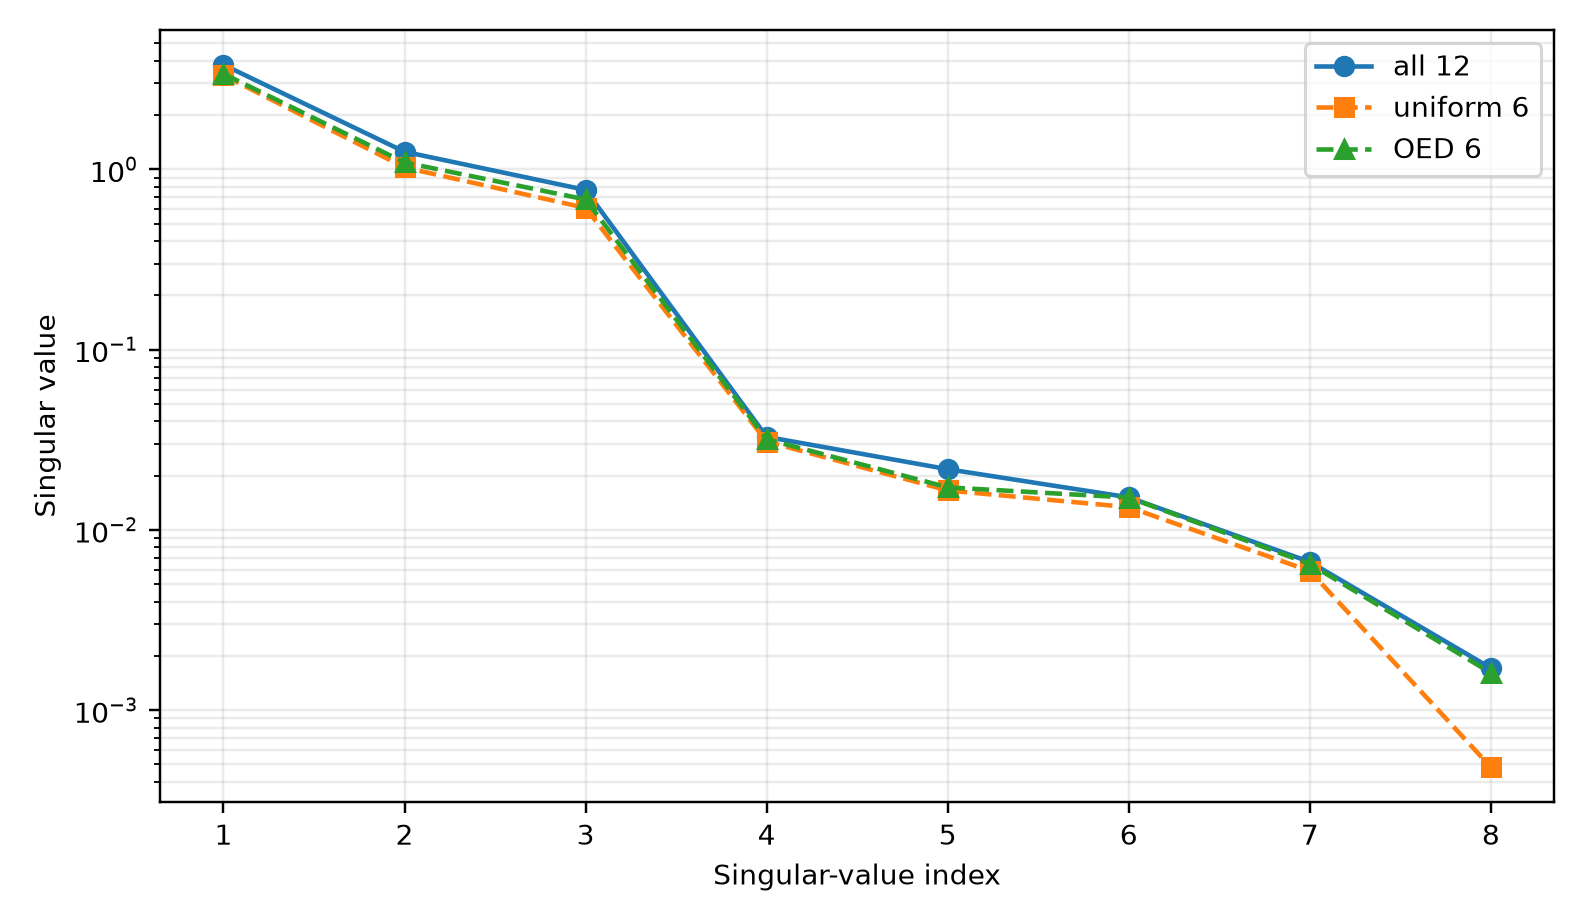
\includegraphics[width=.78\linewidth]{fisher_spectrum_comparison.png}
\caption{全部 12 点、均匀 6 点与 OED 6 点的 Jacobian 奇异值谱。}
\end{figure}

\section{三种参数化与局部反演}
小扰动下
\begin{equation}
\Delta\bm h\approx\bm J\Delta\bm z,
\end{equation}
使用 Tikhonov 正则的局部 Gauss--Newton 解
\begin{equation}
\widehat{\Delta\bm z}=(\bm J^\mathsf{T}\bm J+\lambda\bm I)^{-1}\bm J^\mathsf{T}\Delta\bm h,
\qquad \lambda=2\times10^{-5}.
\end{equation}
比较如下三种方法。

\begin{enumerate}
\item \textbf{full8：}同时估计八个 $z_i$；自由度最高，但最弱方向放大噪声。
\item \textbf{selected4：}穷举四列子集并最大化其 Fisher log-det。当前模型选出 $R_p,L_\sigma,C_g,C_{ps}$；其余参数固定在标称值。
\item \textbf{lowrank4：}取 OED Jacobian 的前四个右奇异向量 $\bm V_4$，令 $\Delta\bm z=\bm V_4\bm a$，只估计四个最可见的参数组合：
\begin{equation}
\hat{\bm a}=\arg\min_{\bm a}\|\bm J\bm V_4\bm a-\Delta\bm h\|_2^2+\lambda\|\bm a\|_2^2.
\end{equation}
\end{enumerate}
selected4 具有直接物理参数名，但忽略了未选参数真实变化；lowrank4 估计的是混合方向，物理命名较弱，却能保留多个参数协同变化对端口的主要影响。

\begin{figure}[htbp]
\centering
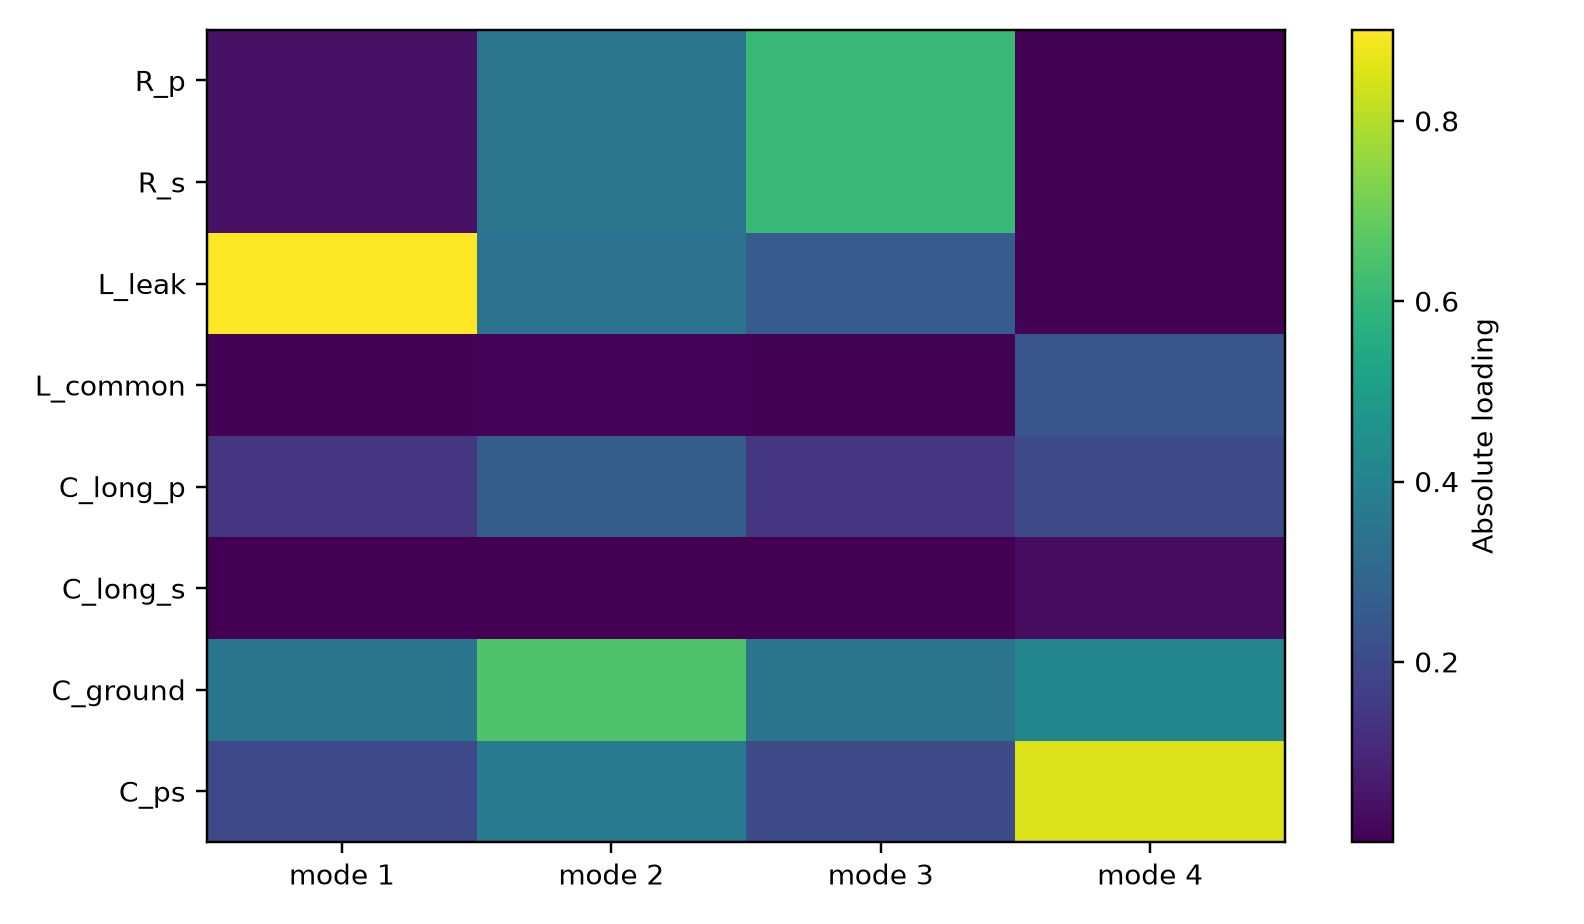
\includegraphics[width=.72\linewidth]{identifiable_lowrank_basis.png}
\caption{四个主可辨识参数方向在八个对数尺度上的绝对载荷。}
\end{figure}

\section{Monte Carlo 设计与结果}
每种频点方案独立生成 100 个样本。八个真实对数参数均匀采样于 $[-0.08,0.08]$，对应正值尺度约在 $[0.923,1.083]$；观测各通道加入标准差 $0.003$ 的高斯噪声。使用非线性精确教师生成真值，但反演采用标称点局部 Jacobian，故结果同时包含噪声与局部线性化误差。随机种子固定为 1709，设备为 NVIDIA GeForce RTX 5070 CUDA。

\begin{table}[htbp]
\centering
\caption{100 次 Monte Carlo 平均结果}
\begin{tabular}{llrrr}
\toprule
频点 & 参数化 & 参数 MAPE & 观测点响应 MAE & 全12点响应 MAE\\
\midrule
均匀6点 & full8 & 11.38\% & $3.59\times10^{-3}$ & $2.32\times10^{-3}$\\
均匀6点 & selected4 & 4.09\% & $2.80\times10^{-3}$ & $1.64\times10^{-3}$\\
均匀6点 & lowrank4 & 3.66\% & $2.92\times10^{-3}$ & $1.70\times10^{-3}$\\
\midrule
OED 6点 & full8 & 12.59\% & $2.58\times10^{-3}$ & $1.55\times10^{-3}$\\
OED 6点 & selected4 & 3.86\% & $1.22\times10^{-3}$ & $7.94\times10^{-4}$\\
OED 6点 & lowrank4 & \textbf{3.20\%} & \textbf{$1.19\times10^{-3}$} & \textbf{$7.76\times10^{-4}$}\\
\bottomrule
\end{tabular}
\end{table}

\begin{figure}[htbp]
\centering
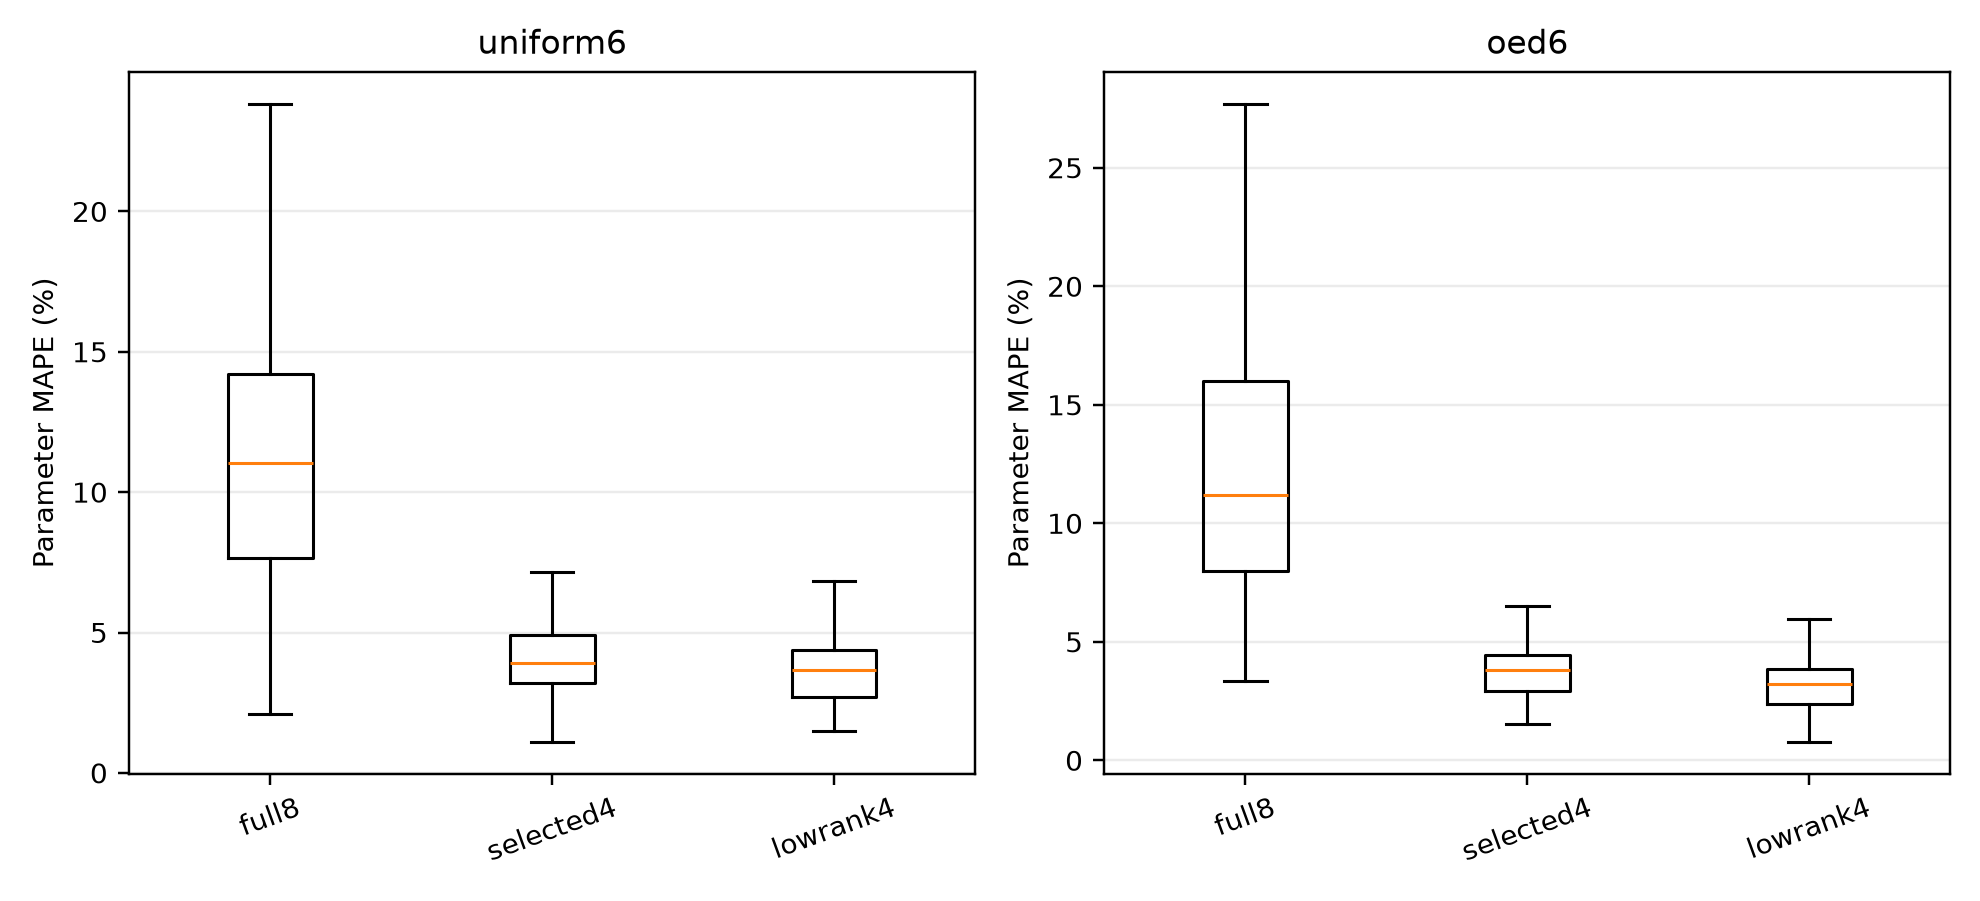
\includegraphics[width=.88\linewidth]{monte_carlo_parameter_error.png}
\caption{不同频点设计和参数化下的参数误差分布。}
\end{figure}

full8 的响应误差仍很小，但参数误差大，说明弱参数之间可以相互补偿。OED 对 full8 的平均参数 MAPE 未优于均匀点，原因是 log-det 优化的是整体局部信息体积，并不保证有限噪声下每个弱原参数的 MAPE 单调下降；但它显著降低响应误差，并把条件数从 6907 降至 2109。参数降维后，OED 优势变得清晰：lowrank4 相对均匀频点的参数 MAPE 从 $3.66\%$ 降至 $3.20\%$，全频响应 MAE 约降低 $54\%$。

\section{证明了什么，没有证明什么}
\subsection*{已经证明}
\begin{itemize}
\item 在当前 EXP-015/016 合成模型中，单个 $Y_{11}$、$Y_{22}$ 或 $Y_{12}$ 不足以稳定区分八个参数，三端口联合观测具有关键互补性。
\item log-det OED 能用 6 个频点获得明显优于均匀 6 点的最小奇异值和条件数。
\item 全八参数响应拟合好不代表参数正确；以 Fisher 选择或主可辨识子空间减少自由度，可显著降低含噪参数误差。
\item 当前最合理的在线目标不是``八参数全部逐一估计''，而是先估计可辨识的少数原参数或低秩组合。
\end{itemize}

\subsection*{尚未证明}
\begin{itemize}
\item 数据是同一 8+8 合成网络生成的，没有真实测量链路、温度漂移、器件寄生、FEM 标签或跨样机变化。
\item 没有引入 DAB 多运行窗口；本实验仅完成端口和频点 OED，不能宣称运行窗口最优。
\item Fisher 结论是标称点附近的局部结论，结构或工况大幅变化后需要重新计算或做鲁棒 OED。
\item lowrank4 的四个坐标是混合物理方向，不能直接解释为四个独立元件故障。
\end{itemize}

\enlargethispage{7\baselineskip}
\section{对后续 GNN 实验的意义}
EXP-016 中 HFT 分型 GNN 未优于同质基线，当前瓶颈不是网络表达力，而是监督目标本身存在病态性。EXP-017 因此建议下一阶段把 AI 目标由八个独立尺度改为：
\begin{equation}
\text{OED 频谱/图结构}\longrightarrow \bm a_{1:4}
\longrightarrow \widehat{\Delta\bm z}=\bm V_4\hat{\bm a},
\end{equation}
或者仅预测 Fisher-selected 参数并把其他参数作为先验/干扰量。只有当复杂前向模型或实测链路产生系统残差时，才让 GNN/频谱网络学习该残差；否则网络只会学习一个本可由线性代数解决的映射。

\section{下一步建议}
第一步，将 EXP-014 的 DAB 多窗口端口电压/电流导出接口与本实验 Fisher 代码连接，计算每个运行窗口的 $\bm W_{r,k}$ 和信息增量；若端口激励矩阵病态，应先选择窗口而非训练网络。第二步，将真实测量噪声协方差替代单位权重，形成加权/鲁棒 OED。第三步，在模型失配数据上比较物理 Gauss--Newton、低秩反演和物理锚定 GNN，而不是继续使用同模生成--同模反演数据宣称 AI 优势。

\section*{复现文件}
主脚本为 \texttt{run\_exp17.py}，自动检查为 \texttt{test\_exp17.py}。\texttt{results/metrics.json} 保存全部指标，\texttt{monte\_carlo\_records.csv} 保存每次误差，\texttt{fisher\_intermediates.npz} 保存原始/归一化 Jacobian、列尺度、低秩基和频点索引。所有数字均可由固定随机种子重新生成。

\end{document}
